\documentclass[TFM.tex]{subfiles}

\begin{document}


%\hyphenation{equi-va-len-cia}\hyphenation{pro-pie-dad}\hyphenation{res-pec-ti-va-men-te}\hyphenation{sub-es-pa-cio}
\chapter{Operads}\label{3}

%Se usan también en tqft, y sirven para construir muchos tipos de álgebras (por ejemplo Lie en característica no 2 por lo de la simetría, asociativas, commutativas, aunque no fields o grupos intuitivamente por la inversa)

In this chapter we define the main object of our study: operads. This object has been gaining importance in mathematics thanks to its ability to encode many kinds of algebras (associative, commutative, Lie...). We begin with the topological version of operads and construct the operad of little disks, which plays the main role in the Deligne conjecture. Topological operads give rise to operads in other categories by taking singular chains or homology. Therefore, we also introduce the concept of operad in a symmetric monoidal category. Finally, we motivate the study of operads and the origin of the Deligne conjecture. We can restrict ourselves to compactly generated Hausdorff spaces when necessary. 




\section{Topological operads}
%First we give the general notion of (topological) operad and some properties of this object.
% EN PRINCIPIO LO DEFINO EN TOP Y YA PREGUNTO SI HACE FALTA QUE SEA EN UNA MONOIDAL SIMÉTRICA. SI HACE FALTA, HACER UNA SECCIÓN DE CATEGORÍAS SIMÉTRICAS MONOIDALES. SI NO, CITAR A DONALD YAU CON QUE SE PUEDE DEFINIR CON MÁS GENERALIDAD
%\url{https://ncatlab.org/nlab/show/operad}
%
%NO PARECE QUE ESTA DEFINICIÓN CAPTURE LA COMPOSICIÓN DEL LITTLE DISKS OPERAD, PERO EN VERDAD SÍ, LO QUE FALTA ES RELLENA CON LA IDENTIDAD HASTA COMPLETAR LA ARIDAD DEL PRIMERO
In the spirit of \cite{May}, an operad is a collection of suitably interrelated spaces $\CC(j)$, whose points are to
be thought of as $j$-ary operations $X^j \to X$ for some topological space $X$. Precisely, we have the following definition.

\begin{defi}\label{operadtop}
An \emph{operad} (also kwown as \emph{symmetric operad}) $\CC$ consists of topological spaces $\CC(j)$ for $j\geq 0$, %with $\CC(0)$ a single point $*$, 
together with the following data:
\begin{enumerate}[(1)]
\item Continuous maps $\gamma : \CC(k) × \CC(j_1) × \cdots × \CC(j_k) \to \CC(\sum_s j_s)$ such that the
following associativity formula is satisfied for all $c\in \CC(k)$, $d_s \in \CC(j_s)$, and $e_t \in \CC(i_t)$:

\[\gamma(
\gamma(c; d_1, \dots , d_k); e_1, \dots , e_j) = 
\gamma(c; f_1, \dots , f_k),
\]
where $$f_s = \gamma(d_s; e_{j_1+\cdots+j_{s−1}+1}, \dots , e_{j_1+\cdots+j_s} ).$$%, and $f_s = *$ if $j_s = 0$ 
These maps are usually called \emph{structure maps}.

\item An identity element $1 \in \CC(1)$ such that 
$\gamma(1; d) = d$ for $d \in \CC(j)$ and 
$\gamma(c; 1,\dots,1) = c$ for
$c \in \CC(k)$.

\item A right action of the symmetric group $\Sigma_j$ on $\CC(j)$ such that the following equivariance
formulas are satisfied for all $c\in \CC(k)$, $d_s \in \CC(j_s)$, $\sigma\in\Sigma_k$, and $\tau_s\in\Sigma_{j_s}$:
\[
\gamma(c\sigma; d_1, \dots , d_k) = 
\gamma(c; d_{\sigma^{−1}(1)}, \dots , d_{\sigma^{−1}(k)})\sigma(j_1, \dots , j_k)
\]
and 
\[
\gamma(c; d_1\tau_1, \dots , d_k\tau_k) = \gamma(c; d_1, \dots , d_k)(\tau_1\oplus\cdots\oplus\tau_k),
\] 
where $\sigma(j_1, \dots , j_k)$ denotes the
permutation of $j$ letters which permutes the $k$ blocks of letters determined by the given
partition of $j$ (a first block of $j_1$, a second one of $j_2$ letters and so on), and $\tau_1\oplus\cdots\oplus\tau_k$ denotes the image of $(\tau_1, \dots , \tau_k)$ under the evident inclusion of $\Sigma_{j_1} × \cdots × \Sigma_{j_k}$ in $\Sigma_j$ (whose image is the corresponding Young subgroup).
%{1,2,...,j} se divide en bloques y se permuta ese conjunto 
\end{enumerate}
\end{defi}

%\url{https://en.wikipedia.org/wiki/Operad_theory}


\begin{defi}
A \emph{morphism} $\psi:\CC \to \CC'$ of operads is a sequence of $\Sigma_j$-equivariant maps  $\psi_j : \CC(j)\to \CC'(j)$ such that
 $\psi_1(1) = 1$ and the following diagram commutes:
 \[
 \begin{tikzcd}
\CC(k)\times \CC(j_1)\times\cdots\times \CC(j_k) \arrow[r, "\gamma"] \arrow[d, "\psi_k\times\psi_{j_1}\times\cdots\psi_{j_k}"'] & \CC(j) \arrow[d, "\psi_j"] \\
\CC'(k)\times \CC'(j_1)\times\cdots\times \CC'(j_k) \arrow[r, "\gamma"]                                                         & \CC'(j)                   
\end{tikzcd}\]
$\Sigma_j$-equivariancy means that $\psi_j(c\sigma)=\psi_j(c)\sigma$ for all $c\in \CC(j)$, $\sigma\in\Sigma_j$ and $j\geq 0$. 
\end{defi}



%\url{https://ncatlab.org/nlab/show/symmetric+monoidal+category#as_algebras_over_the_little_cubes_operad}
% HABLAR ALGO DE ESTAS CATEGORÍAS PARA QUE TENGA MÁS SENTIDO GENERALIZAR LAS DEFINICIONES Y DAR UNA IDEA DE CÓMO SE DEFINEN LAS OPERADS EN ESAS CATEGORÍAS


There is a very visual way to understand operads using trees. Consider a star-shaped tree of $n+1$ leaves, draw one leave pointing downwards and the rest pointing upwards as in the following picture.

\begin{tikzpicture}[line cap=round,line join=round,>=triangle 45,x=1.0cm,y=1.0cm]
\clip(-5.13333333333334,-0.093333333333332) rectangle (12.006666666666668,3.5);
\draw [line width=2.pt] (2.,0.)-- (2.,1.);
\draw [line width=2.pt] (2.,1.)-- (0.3666666666666659,3.);
\draw [line width=2.pt] (2.,1.)-- (1.,3.);
\draw [line width=2.pt] (2.,1.)-- (1.7,3.);
\draw [line width=2.pt] (2.,1.)-- (3.,3.);
\draw (0.1,3.493333333333331) node[anchor=north west] {$1$};
\draw (0.8,3.52) node[anchor=north west] {$2$};
\draw (1.5,3.493333333333331) node[anchor=north west] {$3$};
\draw (2.8,3.453333333333331) node[anchor=north west] {$n$};
\draw (2.1,3.453333333333331) node[anchor=north west] {$\cdots$};
\end{tikzpicture}

These trees are going to be our bricks. Let us call the upward leaves \emph{inputs} and the downward leave \emph{output}. One can interpret a $n$-ary operation as a tree having precisely $n$ inputs and one output. In addition, we can build trees having any number of inputs by grafting the output of a tree into an output of another tree, as in the picture below.

\begin{tikzpicture}[line cap=round,line join=round,>=triangle 45,x=1.0cm,y=1.0cm]
\clip(-2.5333333333333337,-0.7866666666666676) rectangle (11.986666666666668,6.72);
\draw [line width=2.pt] (0.573333333333333,6.093333333333334)-- (1.4,4.6);
\draw [line width=2.pt] (1.4,4.6)-- (1.3866666666666663,6.12);
\draw [line width=2.pt] (1.4,4.6)-- (2.2,6.066666666666667);
\draw [line width=2.pt] (1.4,4.6)-- (1.3866666666666663,3.6533333333333333);
\draw [line width=2.pt] (1.3866666666666663,3.6533333333333333)-- (2.24,2.36);
\draw [line width=2.pt] (2.24,2.36)-- (3.0533333333333332,3.64);
\draw [line width=2.pt] (2.24,2.36)-- (2.24,1.7066666666666663);
\draw [line width=2.pt] (4.96,4.32)-- (5.653333333333333,2.8);
\draw [line width=2.pt] (5.653333333333333,2.8)-- (6.333333333333334,4.253333333333333);
\draw [line width=2.pt] (5.653333333333333,2.8)-- (7.146666666666667,4.133333333333334);
\draw [line width=2.pt] (5.653333333333333,2.8)-- (4.32,4.226666666666667);
\draw [line width=2.pt] (5.653333333333333,2.8)-- (5.586666666666667,4.36);
\draw [line width=2.pt] (5.653333333333333,2.8)-- (5.653333333333333,1.973333333333333);
\draw (4.053333333333334,3.04) node[anchor=north west] {$=$};
\draw [line width=2.pt,dash pattern=on 3pt off 3pt] (1.393433822557186,4.133801401560228) circle (0.6600407206528376cm);
\end{tikzpicture}

This is interpreted as the composition in an operad. Therefore, operadic composition is just grafting trees on the inputs of another tree. It is easier to understand the axioms in these terms. Associativity means that you can graft a tree into another, and graft the result into a third one, or graft the second tree into the third one and then graft the first without changing the final tree as long as we keep track of the inputs where we are grafting the trees. 

The axiom of the unit is the fact that grafting just a stick does not change the shape of the tree (number of inputs). Finally, equivariancy show that we can reorder the inputs before or after grafting as long as keep track of the position of each input before and after the grafting.
%\begin{figure}[h!]
%\begin{tikzpicture}[line cap=round,line join=round,>=triangle 45,x=1.0cm,y=1.0cm]
%\clip(-2.666666666666668,-0.06666666666665) rectangle (15.26666666666667,3.8);
%\draw [line width=2.pt] (5.,0.)-- (5.,1.);
%\draw [line width=2.pt] (5.,1.)-- (4.,2.);
%\draw [line width=2.pt] (5.,1.)-- (6.,2.);
%\draw [line width=2.pt] (4.,2.)-- (3.,3.);
%\draw [line width=2.pt] (4.,2.)-- (4.,3.);
%\draw [line width=2.pt] (4.,2.)-- (5.,3.);
%\draw (2.6666666666666,3.36) node[anchor=north west] {$a$};
%\draw (3.82,3.5) node[anchor=north west] {$b$};
%\draw (4.96,3.36) node[anchor=north west] {$c$};
%\draw (6.,2.4) node[anchor=north west] {$d$};
%\draw (3.4,2.113333333333336) node[anchor=north west] {$abc$};
%\draw (5.04,1.1933333333333358) node[anchor=north west] {$(abc)d$};
%\end{tikzpicture}
%\caption{Operadic composition is denoted as a product. In a binary operation we insert the result of a ternary operation and of an unary operation.}
%\end{figure}

% that one can compose the top three operations with the middle left operation, and then compose the result with the middle right operation, or one can compose the middle operations first, and then insert the three top operations in the appropriate place, giving in both cases the same output. The axiom of the unit element means that $1$ is a neutral element for this product, so we can shrink any edge labelled with $1$. In the picture, equivariancy can be interpreted in the following way: we can change the order of the inputs of the final operation, obtaining $d(abc)$, or we can perform a block transposition on the letters $(abc)d$, which again yields $d(abc)$. 

Operads can also be described by \emph{insertions} (also called \emph{partial compositions} \cite{das})
\[
\circ_i:\CC(p)\times\CC(q)\to \CC(p+q-1),\ 1\leq i\leq p
\]
satisfying 
\[
\begin{cases}
f\circ_i(g\circ_j h)=(f\circ_i g)\circ_{i+j-1} h & 1\leq i\leq p, 1\leq j\leq q\\
(f\circ_j h)\circ_i g=(f\circ_i g)\circ_{j+q-1}h & 1\leq i<j\leq m,
\end{cases}
\]
for $f\in\CC(p)$, $g\in\CC(q)$, $h\in\CC(r)$, and an identity element $1\in\CC(1)$ satisfying $f\circ_i 1=1\circ_1 f=f$ for all $f\in\CC(p)$ and $1\leq i\leq m$. We must also require the equivariance property expressed by the commutativy of the following diagram
\[
\begin{tikzcd}
\CC(p)\times \CC(q)\arrow[r, "\circ_i"]\arrow[d, "\sigma\times\tau"] & \CC(p+q-1)\arrow[d, "\sigma\circ_{\Sigma(i)}\tau"]\\
\CC(p)\times\CC(q)\arrow[r, "\circ_{\Sigma(i)}"] & \CC(p+q-1)
\end{tikzcd}
\]

for all $\sigma\in\Sigma_p$, $\tau\in\Sigma_q$, and where $\sigma\circ_{\Sigma(i)}\tau\in\Sigma_{p+q-1}$ consist of inserting the permutation $\tau$ of the set $\{1,\dots, q\}$ in the place where $\sigma(i)$ is after applying $\sigma$ to the set $\{1,\dots, p\}$, renumbering appropriately. A more detailed explanation of this will be made on section 4.2 chapter 3. The two definitions of operad are related by
\begin{equation}\label{circ}
f\circ_i g=\gamma(f;1,\dots, 1,\underbrace{g}_{i-th},1,\dots, 1)
\end{equation}
and
\[
\gamma(f;g_1,\dots, g_p)= (\cdots((f\circ_1 g_{1})\circ_{k_2} g_{2})\cdots)\circ_{k_p} g_p.
\]
where $g_i\in\CC(n_i)$ and $k_i=1+\sum_{j=1}^{i-1}n_j$.

In fact, defining $\circ_i$ via equation \ref{circ} one can deduce the properties of $\circ_i$ explained before \cite[Chapter 2]{teich}. Therefore, it is more convenient to use the insertion version when possible, as we will do in the next section. 

%ALOMEJOR HACER DIBUJITOS DE LOS AXIOMAS \url{https://en.wikipedia.org/wiki/Operad#\%22Little_something\%22_operads}


\section{Little disks operad}\label{little}
 
 
 Let $E_2(n)$ be the configuration space of $n$ disks $B(x_i,r_i)$ of center $x_i\in D^2$ and radius $r_i\in (0,1]$ (called \emph{little disks}) inside the standard unit disk $D^2$. $E_2(n)$ can be viewed as a subspace of $(D^2\times (0,1])^n$ whose points are of the form $((x_1,r_1),\dots, (x_n,r_n))$ satisfying certain restrictions, namely, $r_i$ must be such that the disk $B(x_i,r_i)\subset D^2$ does not intersect any other disk $B(x_j,r_j)$ and fits inside $D^2$. By convention, $E_2(0)=\{*\}$.  
 
 There is an obvious homotopy equivalence $E_2(n)\simeq \mathcal{M}_2(n)$ from $E_2(n)$ to the configuration space of $n$ points of $D^2$. This homotopy equivalence is given by ``forgetting the radius'' of each little disk. %Hence $\dim H_0(E_2(n))=\dim H_1(E_2(n))=n!$ and $H_i(E_2(n))=0$ for $i>1$.
   Hence $\pi_1(E_2(n))\cong PB_n$, the pure braid group of order $n$, and $\pi_i(E_2(n))=0$ for $i>1$ \cite{fox}. Another consequence of this homotopy equivalence is that the spaces of the little disks operad have the homotopy type of CW-complexes \cite{CW}. Their homology is however rather complicated and it is computed by Cohen et al \cite{cuentas}.  
 
 
\definecolor{xdxdff}{rgb}{0.49019607843137253,0.49019607843137253,1.}

\begin{figure}[h!]
\resizebox{10cm}{4.7cm}{%
\begin{tikzpicture}[line cap=round,line join=round,>=triangle 45,x=1.0cm,y=1.0cm]
\clip(-5.5,-3.4) rectangle (9.5,3.4);
\draw [line width=2.pt,color=xdxdff,fill=xdxdff,fill opacity=0.10000000149011612] (2.,1.) circle (0.7823042886243178cm);
\draw [line width=2.pt,color=xdxdff,fill=xdxdff,fill opacity=0.10000000149011612] (3.,-1.) circle (1.100727032465361cm);
\draw [line width=2.pt,color=xdxdff,fill=xdxdff,fill opacity=0.10000000149011612] (4.48,1.46) circle (0.7496665925596522cm);
\draw [line width=2.pt] (3.,0.) circle (3.1622776601683795cm);
\draw [line width=2.pt] (2.,1.) circle (0.7823042886243178cm);
\draw [line width=2.pt] (4.48,1.46) circle (0.7496665925596522cm);
\draw [line width=2.pt] (3.,-1.) circle (1.100727032465361cm);
\draw (1.84,1.3) node[anchor=north west] {$1$};
\draw (4.32,1.7) node[anchor=north west] {$2$};
\draw (2.8,-0.8) node[anchor=north west] {$3$};
\draw (-1.44,0.6) node[anchor=north west] {\LARGE{$c=$}};
\end{tikzpicture}
}
\caption{A point $c\in E_2(3)$.}
 \end{figure}
 

 
 
 We define for all positive integers $p$ and $q$ and  each $1\leq i\leq p$ the insertion maps 
 \[
 \begin{tikzcd}[row sep=10]
  E_2(p)\times E_2(q)\arrow[r, "\circ_i"] & E_2(p+q-1)\\
  (c_1,c_2)\arrow[r, mapsto, shorten <= 1em, shorten >= 1em] & c_1\circ_i c_2
 \end{tikzcd}
 \]
 by scaling down $c_2$ and inserting it inside $B(x_i,r_i)$, shifting the numbering of the disks of $c_2$ by $i$ as well as shifting the numbering of the disks of $c_1$ with a number greater than $i$ by the number of disks in $c_2$ minus 1, and finally erasing $B(x_i,r_i)$, as shown in the figure below. 
 \begin{figure}[h!]
  \centering
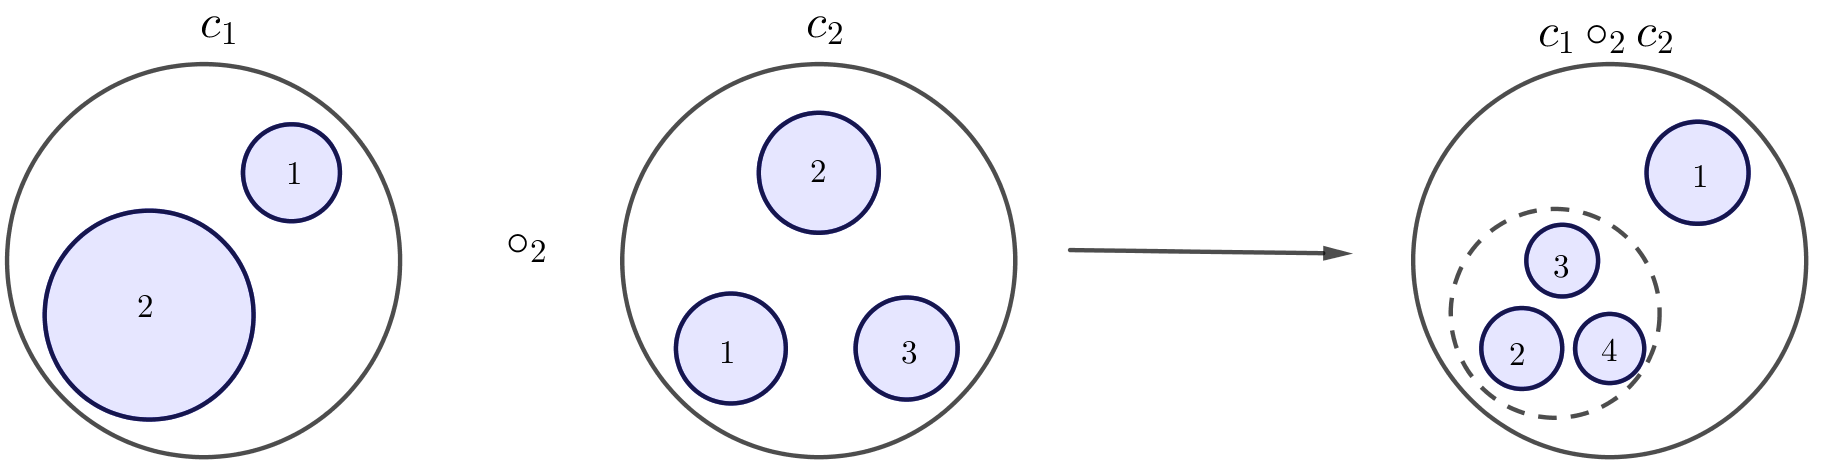
\includegraphics[scale=0.3]{Imagenes/insertion}
\caption{An insertion $\circ_2:E_2(3)\times E_2(3)\to E_2(5)$.}
 \end{figure}
 %\newpage

Note that there is an element $Id_{E_2}\in E_2(1)$ given by the coordinates $(0,1)$ which acts as the identity for this map, since the little disks actually covers the whole disk, so there is no need to rescale anything or shift indices. It is easy to check that these maps satisfy the associativity property of an operad. There is an action $E_2(n)\times \Sigma_n\to E_2(n)$ of the symmetric group on $E_2(n)$ given by reordering the little disks. It is not difficult to check that the maps $\circ_i$ are compatible with this action in the sense of equivariance of operads. Therefore, the familty $E_2=\{E_2(n)\}_{n\geq 0}$ is an operad with identity $Id_{E_2}$ and composition map $\circ_i$. This is what we call the \emph{little disks operad}.



%\begin{remark}
%In the definition of the structure maps we're omitting the disks on which only the identity is acting. If we want to write it with the same notation as we defined operads, the maps should be $\circ_i:E_2(p)\times E_2(q)\times E_2(1)\times\cdots \times E_2(1)\to E_2(p+q-1)$, but since the other spaces act via the identity it is not necessary. In addition, the associativity property of the operad allows us to define every structure maps in terms of the insertions. 
%\end{remark}

\begin{figure}[h!]
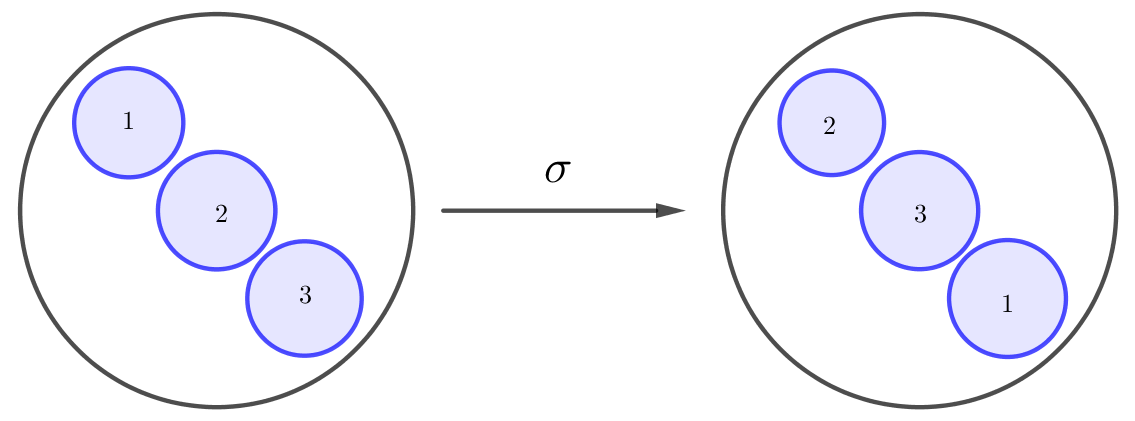
\includegraphics[scale=0.35]{Imagenes//accion}
\caption{Action of $\sigma=(231)$ on a point of $E_2(3)$.}
\end{figure}



\subsection{Action of $E_2$ on a loop space}
Given a based space $(X,x_0)$, consider the loop space $\Omega^2(X)$ of based maps $(S^2, (1,0,0))\to (X, x_0)$. One can interpret this maps as maps $D^2\to X$ sending the boundary $S^1$ of $D^2$ to $x_0$, since they induce a well defined map $D^2/S^1\cong S^2\to X$ and we can choose the quotient map to identify the class of $S^1$ in $D^2/S^1$ with the point $(1,0,0)\in S^2$. 

Now we can define for $n\geq 1$ an action $E_2(n)\times (\Omega^2(X))^n\to \Omega^2(X)$ given by $(c,\gamma_1,\dots, \gamma_n)\mapsto c(\gamma_1,\dots, \gamma_n)$, where 
$c(\gamma_1,\dots, \gamma_n):D^2\to X$ is defined as $\gamma_i$ on the interior of $B(x_i,r_i)$ and to be constantly the base point $x_0$ outside the interior of the little disks. This map has the following immediate properties:
\begin{enumerate}
\item $Id_{E_2}(\gamma)=\gamma$ for all $\gamma\in \Omega^2(X)$.
\item For $c_1\in E_2(p)$ and $c_2\in E_2(q)$, 
$$(c_1\circ_i c_2)(\gamma_1,\dots, \gamma_{p+q-1})=c_1(\gamma_1,\dots, \gamma_{i-1}, c_2(\gamma_i,\dots, \gamma_{i+q-1}),\dots, \gamma_{p+q-1}).$$ 
\item For $c\in E_2(n)$ and $\sigma\in\Sigma_n$, $(c\cdot \sigma)(\gamma_1,\dots,\gamma_n)=c(\gamma_{\sigma^{-1}(1)},\dots, \gamma_{\sigma^{-1}(n)})$. 
\end{enumerate}
Note that for $n=0$, there is only the map $E_2(0)\to\Omega^2(X)$ satisfying $*\mapsto x_0$. 

The action described above turns $\Omega^2(X)$ into an \emph{$E_2$-algebra}. A formal definition of this concept is given below in terms of the \emph{endomorphism operad}. 


\begin{defi}\label{endomorphism}
Let $(X,x)$ be a pointed topological space and define the \emph{endomorphism operad} $\xi_X$ as follows. The product $X^j$ becomes a pointed space with base point $(x,\cdots, x)$. Let $\xi_X(j)$ be the space of based maps $X^j\to X$, $X^0=*$, and $\xi_X(0)$ the inclusion $*\to X$. The data are defined by:
\begin{enumerate}
\item $\gamma(f;g_1,\dots, g_k)=f(g_1\times\cdots\times g_k)$ for $f\in \xi_X(k)$ and $g_s\in\xi_X(j_s)$ such that $\sum_s j_s=j$.
\item The identity element $1_X\in\xi_X(1)$ is the identity map on $X$.
\item $(f\sigma)(y)=f(\sigma y)$ for $f\in\xi_X(j)$, $\sigma\in\Sigma_j$ and $y\in X^j$, where $\Sigma_j$ acts on $X^j$ by $\sigma(x_1,\dots, x_j)=(x_{\sigma^{-1}(1)},\dots, x_{\sigma^{-1}(j)})$. 
\end{enumerate}

Given a morphism of operads $\CC\to \xi_X$, we say that the pair $(X,\CC)$ is an \emph{$\CC$-algebra} (sometimes called \emph{$\CC$-space} \cite{May}). Algebras over operads can also be described in terms of insertions, obtaining a definition whose axioms are the properties of the action of $E_2$ on $\Omega^2(X)$ we described before.
\end{defi}


Note that giving a morphism $\CC\to \xi_X$ is equivalent to giving a sequence of maps $\CC(k)\times X^k\to X$, so this definition is consistent with saying that $\Omega^2(X)$ is an $E_2$-algebra. 





%PREGUNTARLE QUÉ SENTIDO TIENE SER QUASI-ISOMORFO A LA HOMOLOGÍA, SI LA HOMOLOGÍA DE LA HOMOLOGÍA ES 0
%
%CON LO DEL SUSTITUTO, SI TIENE LA MISMA HOMOLOGÍA QUE C2, ENTONCES CONSIGUES QUE C(SUSTITUTO) ACTÚE EN H(A,A), PERO DE AHÍ EN PRINCIPIO NO SE SACA LA ACCION EN C(A,A)
\subsection{Little $k$-disks operad}\label{intervals}

One can define an operad $E_k$ for $k\geq 0$ in the same way we've defined $E_2$, but replacing the 2-dimensional disks by $k$-dimensional disks. Their action on $\Omega^k(X)$ is defined similarly. For $k\geq 2$, $E_k$ gives rise to more topologically rich spaces, since they have non trivial homotopy groups in dimensions greater than $1$, and there is also an operad $E_\infty$ (see \cite{cuentas}). 

The case $k=1$ is particularly simple. For $E_1$, usually called \emph{little intervals operad}, we have the following proposition.

\begin{prop}\label{E1}
For all $n\geq 0$, $E_1(n)$ is a disjoint union of contractible spaces.
\end{prop}
\begin{proof}
The case $n=0$ is trivial so take $n>0$. Each component of $E_1(n)$ corresponds to a fixed ordering of the intervals i.e. a certain permutation $\sigma\in\Sigma_n$ acting on the canonical increasing order. This is because no path can switch two little intervals inside $[0,1]$ without intersecting them. Since there is a homotopy equivalence from $E_1(n)$ to the configuration space of $n$ points in $[0,1]$, we can apply this homotopy to each of the components, obtaining that each component is homotopy equivalent to one of the following spaces
\[
\{(x_{\sigma(1)},\dots, x_{\sigma(n)})\in (0,1)^n\mid x_{\sigma(1)}<\dots< x_{\sigma(n)}\}
\]
for each $\sigma\in\Sigma_n$ (the same $\sigma$ that gives us the corresponding component acting on the increasing order).
 We prove that these spaces are contractible. For simplicity, we show it for the trivial permutation. Let us denote $\mathcal{M}_1(n)=\{(x_{1},\dots, x_{n})\in (0,1)^n\mid x_{1}<\dots< x_{n}\}$.
%We have that $E_1(n)\simeq \mathcal{M}_1(n)$ via the analogue of homotopy equivalence $E_2(n)\simeq\mathcal{M}_2(n)$.  Therefore, we've reduced the proof to show that the configuration space of $n$ points of $(0,1)$, $\mathcal{M}_1(n)$, is contractible. Any point $(x_1,\dots, x_n)\in\mathcal{M}_1(n)$ is a sequence of distinct points of $(0,1)$, so we can order them and consider the sequence $0<x_{i_1}<\cdots<x_{i_n}<1$.

%We have that the space $\{(x_{\sigma(1)},\dots, x_{\sigma(n)}\in (0,1)^n\mid x_{\sigma(1)}<\dots< x_{\sigma(n)}\}$  is precisely the configuration space $\mathcal{M}_1(n)$. Let $p=\left(\frac{1}{n+1},\dots, \frac{n}{n+1}\right)\in \mathcal{M}_1(n)$. 
 Let $p=\left(\frac{1}{n+1},\dots, \frac{n}{n+1}\right)\in \mathcal{M}_1(n)$.  We now show that the map $q:\mathcal{M}_1(n)\to \{p\}$ defined on each coordinate by $x_{i}\mapsto \frac{i}{n+1}$ (so that every point maps to $p$) is an homotopy equivalence with the inclusion $i:\{p\}\hookrightarrow \mathcal{M}_1(n)$ as homotopy inverse. We define a homotopy $\mathcal{M}_1(n)\times [0,1]\to \mathcal{M}_1(n)$ between $Id_{\mathcal{M}_1(n)}$ and $i\circ q$ as $(x,t)\mapsto (1-t)x+tp$. Since $[0,1]$ is convex, this yield a well-defined map $(0,1)^n\times [0,1]\to (0,1)^n$. We need to check that it preserves the order of the coordinates. 
 That is easy since if $x_{i}<x_{j}$, then clearly 
\[
(1-t)x_{i}+t\frac{i}{n+1}<(1-t)x_{j}+t\frac{j}{n+1}
\] 
Continuity is obvious so we've defined the desired a homotopy.
\end{proof}

Because of this property of $E_1$ one sometimes consider the \emph{non-symmetric} or non-$\Sigma$ operad $E_1$, defined similarly but we require the centers of the intervals to have be in increasing order. This is the same as selecting one of the components of the equivariant $E_1$, so the non-symmetric operad is contractible. 






%ESTO ES INTERESANTE, LO DEJO AQUÍ \url{https://amathew.wordpress.com/2011/11/13/operads-i/}

\section{Operads in symmetric monoidal categories}
We've treated operads only in the category of topological spaces, but they can be defined in a more general setting, namely, in any \emph{symmetric monoidal category} \cite{Yau}. We're going to introduce this categories since it becomes more natural to talk about operads and other constructions in other categories having that framework in advance.

\begin{defi}\label{monoidal}
A \emph{symmetric monoidal category} is a category $\mathscr{M}$ equipped with:
\begin{enumerate}[(1)]
\item A functor $\otimes: \mathscr{M}\times \mathscr{M}\to \mathscr{M}$ called the \emph{tensor product}.
\item An object $I\in \mathscr{M}$ called the \emph{unit}.
\item Natural isomorphism $a_{x,y,z} : (x \otimes y) \otimes z \to x \otimes (y \otimes z)$ (called the \emph{associator}), $\lambda_x : I \otimes x \to x$ (\emph{left unitor}), $\rho_x : x \otimes I \to x$ (\emph{right unitor}) and $B_{x,y}: x\otimes y\to y\otimes x$ (\emph{braiding}).
\end{enumerate}

We demand the following that the following diagram of unit coherence commutes:
\[
\begin{tikzcd}
x\otimes I\arrow[r, "B_{x,I}"]\arrow[d, "\rho_x"']& I\otimes x\arrow[dl, "\lambda_x"]\\
x & 
\end{tikzcd}
\]

We also demand that the associator and unitors obey the triangle identity, which says this diagram commutes:
\[
\begin{tikzcd}
(x\otimes I)\otimes y \arrow[rr, "{a_{x,I,y}}"] \arrow[rd, "\rho_x\otimes 1_y"'] &            & x\otimes (I\otimes y) \arrow[ld, "1_x\otimes\lambda_y"] \\
& x\otimes y &                                                        
\end{tikzcd}
\]

We demand that the associator obey the pentagon identity, which says this diagram commutes:

\[
\begin{tikzcd}[column sep=-25, row sep=35]
                                                                                                            &                                                                     & (w\otimes x)\otimes (y\otimes z) \arrow[rrd, "{a_{w,x,y\otimes z}}"] &                                                                         &                                \\
((w\otimes x)\otimes y)\otimes z \arrow[rru, "{a_{w\otimes x,y,z}}"] \arrow[rdd, "{a_{w,x,y}\otimes 1_z}"'] &                                                                     &                                                                      &                                                                         & w\otimes(x\otimes(y\otimes z)) \\
                                                                                                            &                                                                     &                                                                      &                                                                         &                                \\
                                                                                                            & (w\otimes (x\otimes y))\otimes z \arrow[rr, "{a_{w,x\otimes y,z}}"] &                                                                      & w\otimes ((x\otimes y)\otimes z) \arrow[ruu, "{1_w\otimes a_{x,y,z}}"'] &                               
\end{tikzcd}
\]


We demand that the braiding and associator obey the hexagon identity:
\[
\begin{tikzcd}
(x\otimes y)\otimes z \arrow[r, "{a_{x,y,z}}"] \arrow[d, "{B_{x,y}\otimes 1_z}"'] & x\otimes (y\otimes z) \arrow[r, "{B_{x,y\otimes z}}"]   & (y\otimes z)\otimes x \arrow[d, "{a_{y,z,x}}"] \\
(y\otimes x)\otimes z \arrow[r, "{a_{y,x,z}}"]                                    & y\otimes (x\otimes z) \arrow[r, "{1_y\otimes B_{x,z}}"] & y\otimes (z\otimes x)                         
\end{tikzcd}
\]
And lastly, we demand that $B_{y,x}B_{x,y}=1_{x\otimes y}$.
\end{defi}

If we drop the braiding from the definition above we obtain what is simply called a \emph{monoidal category}. If we omit the constraint $B_{y,x}B_{x,y}=1_{x\otimes y}$, then we can get a \emph{braided monoidal category}. In that case we have to add the following diagram, which is deduced from the hexagon identity and the equality $B_{y,x}B_{x,y}=1_{x\otimes y}$ in the case of symmetric monoidal categories:
\[
\begin{tikzcd}
	x\otimes (y\otimes z) \arrow[r, "{a^{-1}_{x,y,z}}"] \arrow[d, "{1_x\otimes B_{y,z}}"'] & (x\otimes y)\otimes z \arrow[r, "{B_{x\otimes y, z}}"]   & (y\otimes z)\otimes x \arrow[d, "{a^{-1}_{z,x,y}}"] \\
	x\otimes (z\otimes y) \arrow[r, "{a^{-1}_{x,z,y}}"]                                    & (x\otimes z)\otimes y \arrow[r, "{B_{x,z}\otimes 1_y}"] & (z\otimes x)\otimes y                         
\end{tikzcd}
\]
\begin{ex}\
\begin{enumerate}
\item The categories $\Set$ and $\Top$ are symmetric monoidal categories with the cartesian product as tensor product and a singleton as unit.

\item The category of $k$-modules and the category of $k$-algebras have obvious tensor structures that can be used in the graded case too, though it is more common to introduce the Koszul sign convention in the braiding.  
\item If $k$ is a field, the category $\Vect_k$ of $k$-vector spaces carries the standard structure of a monoidal category coming from the tensor product (over $k$) of vector spaces. The standard braiding that identifies $V\otimes W$ with $W\otimes V$ by mapping elements $v\otimes w$ to $w\otimes v$ obviously makes $\Vect_k$ into a symmetric monoidal category. This is also true for the category $\Vectgr_k$ of graded vector spaces over $k$ (again, with the sign convention).

 %, but this tensor structure is not symmetric in general. Some cases where it is symmetric are $k=\Z_m$ and $k=\Q$. %en la tabla de caracteres de Z_2xZ_2 se ve que TRIVxAlT tiene que ser distinta a ALTxTRIV, como las representaciones son A-modulos para A el álgebra del grupo, se tiene lo que he dicho




\item The category of chain complexes of $k$-modules, $\Ch(k\Mod)$, can be endowed with a structure of symmetric monoidal category defining the following thensor structure. For chain complexes $X,Y\in\Ch(k\Mod)$ write $X\otimes Y$ for the chain complex whose component of degree $n$ is given by the direct sum
\[
(X \otimes Y)_n := \bigoplus_{i + j = n} X_i \otimes_R Y_j
\]
and whose differential is given on elements $x\otimes y$ of homogeneous degree by
\[
\partial^{X \otimes Y} (x\otimes y) = \partial^X x\otimes y + 
  (-1)^{\deg(x)} x\otimes\partial^Y y
  \,.
\]
The unit object is the chain complex concentrated in degree 0 on the tensor unit $k$ of $k\Mod$. Operads in this category are usually called \emph{$dg$-operads} (differential graded operads). 

\item The category $\SSet$ of simplicial sets has a very simple monoidal structure. Given two simplicial sets $S$ and $T$ regarded as functors $\mathbf{\Delta}^{op}\to\Set$, we can define $S\otimes T=S\times T$, meaning that $S\otimes T:[n]\mapsto S_n\times T_n$ and send the morphisms to the obvious ones. The unit in this category is the simplicial set $X_n=\{*\}$ for all $n$ and identities as face and degeneracy maps. 

\item The category $\Cat$ of small categories (the collection of objects and the collection of morphisms are both sets) is symmetric monoidal with the product of categories and the category with one object and only the identity morphism as unit. %el objeto terminal es el producto vacío

\item  More generally, any category with finite categorical products is symmetric monoidal with its product as tensor product and the terminal object as unit. This monoidal structures are called \emph{cartesian} structures.
\end{enumerate}



\end{ex}


% The precise definition(LAX) MONOIDAL FUNCTORS \url{https://ncatlab.org/nlab/show/monoidal+functor} SI ME LO PUEDO AHORRAR ME LO AHORRO

For an arbitrary symmetric monoidal category $\mathscr{M}$ we obtain the following definition of operad, which specializes to the definition \ref{operadtop} for $\mathscr{M}=\Top$.

\begin{defi}
Let $\mathscr{M}$ be a symmetric monoidal category. A (\emph{symmetric}) \emph{operad} in $\mathscr{M}$ consists of objects $\OO(n)$ of $\mathscr{M}$ indexed over the natural numbers equipped with the following extra structure: 

\begin{enumerate}
\item Left actions of opposite symmetric groups $ρ_n^{op}:\Sigma_n^{op}→\Hom(\OO(n),\OO(n))$.
\item A \emph{unit} $e:I→\OO(1)$ (which we think of as picking out the identity). %Right del opposite es lo mismo que left del normal https://en.wikipedia.org/wiki/Opposite_group el motivo es que ya había puesto que fueran a la derecha y habría tenido que cambiar mucho
\item Composition operations
\[
\OO(k) \otimes \OO(n_1) \otimes \cdots \otimes \OO(n_k) \xrightarrow{\gamma} \OO(n_1 + \ldots + n_k)
\]
These data are subject to following axioms that can be found in \cite{Yau} and \cite{tesis}.
\begin{itemize}
\item For $n=\sum_{i=1}^k n_i$, $j=\sum_{i=1}^n j_i$, $g_s=\sum_{i=1}^sn_i$ and $h_s=j_{g_s-1}+\cdots j_{g_s}$ ($1\leq s\leq k$), the following diagram of associativity commutes %el 1 es la identidad
\[
\begin{tikzcd}
\OO(k)\otimes\left(\bigotimes_{i=1}^k\OO(n_i)\right)\otimes\left(\bigotimes_{r=1}^n\OO(j_r)\right)\arrow[dd, "\text{permute with the symmetry constraint}"']\arrow[r, "\gamma\otimes 1^j"] & 
\OO(n)\otimes \left(\bigotimes_{i=1}^n\OO(j_i)\right)\arrow[d, "\gamma"]\\
& \OO(j)\\
\OO(k)\otimes \bigotimes_{s=1}^k\left[\OO(n_s)\otimes\left(\bigotimes_{q=1}^{n_s}\OO(j_{g_{s-1+q}})\right)\right]\arrow[r, "1\otimes \gamma^n"] & 
\OO(k)\otimes \left(\bigotimes_{s=1}^k\OO(h_s)\right)\arrow[u, "\gamma"]
\end{tikzcd}
\]
\item The following unitality diagrams commute
\[
\begin{tikzcd}
\OO(k)\otimes I^{\otimes k} \arrow[d, "1\otimes e^k"'] \arrow[r, "\cong"] & \OO(k) & I^{\otimes k}\otimes \OO(k) \arrow[d, "e \otimes 1"'] \arrow[r, "\cong"] & \OO(k) \\
\OO(k)\otimes\OO(1)^{\otimes k} \arrow[ru, "\gamma"']                     &        & \OO(1)^{\otimes k}\otimes\OO(k) \arrow[ru, "\gamma"']           &       
\end{tikzcd}
\]
\item Finally, the following diagrams expresing $\Sigma_n$-equivariance also commute
\[
\begin{tikzcd}[column sep =80]
\OO(k)\otimes \OO(n_1)\otimes \cdots \otimes \OO(n_k)\arrow[d, "\gamma"] \arrow[r, outer sep=4pt, "\sigma\otimes(\text{reorder with symm. const.})"]& \OO(k)\otimes\OO(n_{\sigma(1)})\otimes\cdots\otimes \OO(n_{\sigma(k)})\arrow[d, "\gamma"]\\
\OO(n) \arrow[r, "{\sigma(n_{\sigma(1)},\dots,n_{\sigma(k)})}"]& \OO(n)
\end{tikzcd}
\]
and
\[
\begin{tikzcd}
\OO(k)\otimes \OO(n_1)\otimes \cdots \otimes \OO(n_k)\arrow[r, "1\otimes \tau_1\otimes\cdots\tau_k"]\arrow[d, "\gamma"] & \OO(k)\otimes\OO(n_1))\otimes\cdots\otimes \OO(n_k)\arrow[d,"\gamma"]\\
\OO(n)\arrow[r, "\tau_1\oplus\cdots\oplus\tau_k"] & \OO(n)
\end{tikzcd}
\]
where for $\sigma\in\Sigma_k$, $\tau_s\in\Sigma_{n_s}$, then $\sigma(n_1,\dots, n_k)\in\Sigma_n$ permutes $k$ blocks $(1,\dots, n_1),\dots, (n_{k-1}+1,\dots, n_k)$ via $\sigma$ and $\tau_1\oplus\cdots\oplus\tau_k$ is the block sum of permutations.
\end{itemize}

%identities such as associativity and unitality of composition, and compatibility of composition with symmetric group actions. For example, the unit laws say that the composite
%\[
%\OO(n) \cong I^{\otimes n} \otimes \OO(n) \xrightarrow{e^{\otimes n} \otimes 1} \OO(1)^{\otimes n} \otimes \OO(n) \xrightarrow{\gamma} \OO(n)
%\]
%is the identity map, as is
%\[
%\OO(n) \cong \OO(n) \otimes I^{\otimes n} \xrightarrow{1 \otimes e^{\otimes n}} \OO(n) \otimes \OO(1)^{\otimes n} \xrightarrow{\gamma} \OO(n)
%\] 
%The reader is referred to page 194 of \cite{Yau} and to \cite{tesis} to see the diagrams associated to the axioms.  PUEDO COGERLO DE LA TESIS PARA COMPLETARLO SI TENGO TIEMPO
\end{enumerate}

%\url{https://ncatlab.org/nlab/show/operad}


\end{defi}

A non-symmetric (or non-$\Sigma$) version is obtained by dropping out the right action of the symmetric group. %or equivalently%, by declaring it to be trivial. 
If we furthermore insist that $\OO(0)=I$, then the operad is called \emph{unital}. In most cases we won't need to use the categorical definition since normaly one can just mimic the definition \ref{operadtop}.


\begin{defi}
Let $\OO$ and $\mathcal{P}$ be operads in $\mathscr{M}$. A map of operads $f:\OO\to \mathcal{P}$ is a collection of maps $\OO(n)\to \mathcal{P}(n)$ such that the following conditions hold:
\begin{enumerate}
\item Compatibility with units:  $f\circ e_\OO=e_\mathcal{P}$, where $e_\OO$ and $e_\mathcal{P}$ are the units.
\item Compatibility with operad compositions: $f\circ \gamma_\OO=\gamma_\mathcal{P}\circ (f\otimes\cdots\otimes f)$ where $\gamma_\OO$ and $\gamma_\mathcal{P}$ are the structure maps and the tensor product $f\otimes\cdots\otimes f$ is taken as many times as the number of arguments of $\gamma_\mathcal{P}$. 
\item  Compatibility with the action of the symmetric groups: $f\circ \rho_\OO(\sigma)=\rho_\mathcal{P}(\sigma)\circ f$ for every and $\sigma\in\Sigma_n$ and for all $n$, where $\rho_\OO$ and $\rho_\mathcal{P}$ are the actions of $\Sigma_n^{op}$ on $\OO$ and $\mathcal{P}$, respectively.
\end{enumerate}
\end{defi}



If we work in a symmetric monoidal closed category (a closed category is, roughly speaking, a category where each hom-set can be regarded as an object of the category, see \cite[\textsection 6.1]{handbook}) there is also an \emph{endomorphism operad} $\xi_X$ for each $X$ in the symmetric monoidal category $\mathscr{M}$ with unit $I$. The $j$-th component $\xi_X(j)$ is just $\Hom(X^{\otimes j},X)$ and the identity of the operad is the map $1_x:I\to \Hom(X,X)$ that sends $I$ to the identity on $X$. The composition map and the action of the symmetric group is defined analogously to the definition \ref{endomorphism}. Therefore, one can define the notion of \emph{algebra over an operad} $\OO$ as an object $X$ equipped with an operad map $\xi:\OO\to\xi_X$. Alternatively, the data of an $\OO$-algebra is given by a sequence of maps
%la categoría Top no es cartesian closed (así que esta noción de operad de endomorfismos realmente no es la de arriba), pero sí los compactly generated Hausdorff. Las otras categoráis que uso son monoidal closed
\[
\OO(j) \otimes X^{\otimes j} \to X
\]
which specifies an action of $\OO$ via finitary operations on $X$, with compatibility conditions between the operad multiplication and the structure of plugging in $j$ finitary operations on $X$ into a $j$-ary operation (and compatibility with actions by permutations). This alternative definition is possible due to the well-known tensor-hom adjuntion, i.e., the isomorphism $\Hom(X\otimes Y,Z)\cong \Hom(X,\Hom(Y,Z))$ \cite{tensor-hom}. 

Note that a map of operads $\OO\to \OO'$ endows an $\OO'$-algebra with a canonical $\OO$-algebra structure.

\begin{defi}
	A \emph{morphism} of $\OO$-algebras $X$ and $Y$ is a family of morphisms $f:X\to Y$ compatible with the action of $\OO$ in the sense that the following diagram commutes for all $j$
	\[
	\begin{tikzcd}
	\OO(j)\otimes X^{\otimes j}\arrow[r, "Id\otimes f^{\otimes j}"]\arrow[d] & 	\OO(j)\otimes Y^{\otimes j}\arrow[d]\\
	X\arrow[r, "f"] & Y
	\end{tikzcd}
	\]
	\end{defi}

 %el converse puede ser que el functor de p-algebras a p'-algebras admite left adjoint que es pag 140 de AlgebraicOperads %The converse is also obviously true: in order to define a map of operads it is enough to endow any $\OO'$-algebra with a canonical $\OO$-algebra structure. 

For a functor $F:\mathscr{M}\to\mathscr{N}$ between monoidal categories, we would like $F$ to preserve the tensor structures so that we can send operads to operads. In most cases, it will be enough to have  morphisms $1_{\mathscr{N}}\to F(1_\mathscr{M})$ and $F(A\otimes_{\mathscr{M}}B)\to F(A)\otimes_{\mathscr{N}} F(B)$ satisfying some natural associativity and unitality properties (see \cite[Definition 6.4.1]{handbook}). Functors fulfilling that last property are called \emph{lax monoidal}. We give an example of a lax monoidal functor in the next section. When the morphisms before are isomorphisms, and hence $F$ preserves the monoidal structure, then $F$ is simply called \emph{monoidal}.

\subsection{Connection between $E_2$ and Gerstenhaber algebras}\label{zilber}

Now that we've defined operads in a more general context, we're ready to draw the connection between the $E_2$ operad and the Gerstenhaber algebras. Since $E_2=\{E_2(n)\}_{n\geq 0}$ is a collection of topological spaces, one can consider the collection of singular chain complexes $C_*(E_2)=\{C_*(E_2(n))\}_{n\geq 0}$ over the fixed ring $k$ (for our purposes $k=\Q$). This family is an operad of chain complexes making use of the \emph{Eilenber-Zilber map} \cite{EZ} $C_*(X)\otimes C_*(Y)\to C_*(X\times Y)$ for arbitrary topological spaces $X$ and $Y$. 

In first place, note that an action of the symmetric group $\rho:X\times\Sigma_n\to X$ can be seen as a family of continuous maps $\rho_\sigma:X\to X$ for each $\sigma\in\Sigma_n$, so they induce an action $\rho_*: C_*(X)\times\Sigma_n\to C_*(X)$. %también hay una acción natural reordenando los vértices del símplice o del cubo 

Next, in order to properly define the Eilenberg-Zilber map explicitly, we have to construct the singular chain complex in two steps. First, consider the simplicial set $S^{sing}(X)$ whose $n$-simplices are just $n$-singular simplices $\sigma:\Delta^n\to X$. The face and degenerancy maps $d_i$ and $s_i$ are obtained from the corresponding $d^i:\Delta^{n-1}\to \Delta^{n}$ and $s^i:\Delta^n\to\Delta^{n-1}$ by composition i.e. $d_i(\sigma)=\sigma\circ d^i$ and $s_i(\sigma)=\sigma\circ s^i$. Then, one defines $C_*(X)=C(S^{sing}(X))$, the chain complex of vector spaces, where the degree $n$-component is generated by the $n$-simplices and the differentials are the usual alternate sums $d=\sum_{i=0}^{n-1}(-1)^id_i$. This definition of $C(\cdot)$ actually admits any simplicial set. Note that this functor factors through another functor which transforms $S^{sing}(X)$ into a simplicial abelian group or a simplicial vector space.

Recall that the product $\Delta^p\times\Delta^q$ can be triangulated in such a way that $\Delta^{p+q}\subset \Delta^p\times\Delta^q$ \cite[Proof of Theorem 2.10]{Hatcher} (to avoid choosing a particular inclusion, one can instead consider singular cubes $f:[0,1]^p\to X$, for which we have $[0,1]^p\times [0,1]^q=[0,1]^{p+q}$). Therefore, one can take two singular simplices $f:\Delta^p\to X$ and $g:\Delta^q\to X$ and define their product $f\otimes g$ as the restriction of $f\times g$ to $\Delta^{p+q}$. Now we give the following definition:

\begin{defi}
The \emph{Eilenberg-Zilber map} is the natural transformation on chain complexes
\[
\nabla :  C_p(X) \otimes C_q(X) \to C_{p+q}(X \times Y)
\]
defined on $a\in C_p(X)$ and $b\in C_q(Y)$ by 
\[
\nabla : a \otimes b \mapsto 
   \sum_{(\mu,\nu)} sign(\mu,\nu) s_\nu(a) \otimes s_\mu(b)
\]
where the sum is over all $(p,q)$-shuffles
\[
(\mu,\nu) = (\mu_1, \cdots, \mu_p, \nu_1, \cdots, \nu_q),
\]
i.e. permutations $\sigma\in\Sigma_{p+q}$ such that $$\sigma(1)=\mu_1<\cdots<\sigma(p)=\mu_p$$ and $$\sigma(p+1)=\nu_1<\cdots<\sigma(p+q)=\nu_q.$$ The corresponding degeneracy maps are
\[
s_{\mu} = s_{\mu_p - 1} \circ \cdots s_{\mu_2 - 1} \circ s_{\mu_1 - 1}
\]
and
\[
s_{\nu} = s_{\nu_q - 1} \circ \cdots s_{\nu_2 - 1} \circ s_{\nu_1 - 1}
\]
\end{defi}
The shift in the indices is to be coherent with the convention that the shuffle $(μ,ν)$ is a permutation of $\{1,\dots,p+q\}$. It is straightforward to show that this map is a map of chain complexes. We now prove that $\nabla$ is associative, which is needed in order to an operadic structure be induced in $C_*(E_2)$ from the one in $E_2$. It is also necessary to show that $\nabla$ is commutative, but we will not do that here.

\begin{lemma}
The Eilenberg-Zilberg map $\nabla$ is associative, i.e. the following diagram commutes
\[
\begin{tikzcd}
C_p(X)\otimes C_q(Y)\otimes C_r(Z)\arrow[r, "\nabla\otimes 1"]\arrow[d, "1\otimes\nabla"] & C_{p+q}(X\times Y)\otimes C_r(Z)\arrow[d,"\nabla"]\\
C_p(X)\otimes C_{q+r}(Y\times Z)\arrow[r, "\nabla"] & C_{p+q+r}(X\times Y\times Z)
\end{tikzcd}
\]
for arbitrary spaces $X$, $Y$ and $Z$. 
\end{lemma} 

\begin{proof}
The technique used in this proof is inspired by the proof of \cite[Lemma 2.9]{Madsen}. Let us denote $S(p,q)$ the set of all $(p,q)$-shuffles and $S(p,q,r)$ the set of permutations $\sigma\in\Sigma_{p+q+r}$ such that 
\begin{gather*}
\sigma(1)<\cdots<\sigma(p)\\
\sigma(p+1)<\cdots<\sigma(p+q)\\
\sigma(p+q+1)<\cdots<\sigma(p+q+r)
\end{gather*}
We will also need the subsets $S(\overline{p},q,r)$ and $S(p,q,\overline{r})$, where $\sigma\in S(\overline{p},q,r)$ if and only if $\sigma\in S(p,q,r)$ and $\sigma$ is the identity on $\{1,\dots, p\}$, and where $\sigma\in S(p,q,\overline{r})$ if and only if $\sigma\in S(p,q,r)$ and $\sigma$ is the identity on $\{p+q+1,\dots, p+q+r\}$.

Permutations in $S(\overline{p},q,r)$ or $S(p,q,\overline{r})$ can also be denoted by $(\mu,\nu,\delta)$ in a similar fashion to how we denoted $(p,q)$-shuffles in the definition of $\nabla$. 

There are bijections
\begin{equation}\label{bijections}
\begin{aligned}
S(p,q+r)\times &S(\overline{p},q,r)\longrightarrow S(p,q,r)\\
&(\sigma,\tau)\longmapsto \sigma\tau\\
\\
S(p+q,r)\times &S(p,q,\overline{r})\longrightarrow S(p,q,r)\\
&(\sigma,\tau)\longmapsto \sigma\tau
\end{aligned}
\end{equation}
With these notations we have
\begin{align*}
\nabla(\nabla(a\otimes b)\otimes c)=&\nabla\left(\left(\sum_{(\mu,\nu)\in S(p,q)} sign(\mu,\nu) s_\nu(a) \otimes s_\mu(b)\right)\otimes c\right)\\
=& \sum_{(\eta,\gamma)\in S(p+q,r)}sign(\eta,\gamma)s_\gamma\left(\sum_{(\mu,\nu)\in S(p,q)} sign(\mu,\nu) s_\nu(a) \otimes s_\mu(b)\right)\otimes s_\eta(c)\\
=&\sum_{(\eta,\gamma)\in S(p+q,r)}sign(\eta,\gamma)\sum_{(\mu,\nu)\in S(p,q)} sign(\mu,\nu) s_\gamma(s_\nu(a) \otimes s_\mu(b))\otimes s_\eta(c).\\
\end{align*}
Now, since for a degenerancy map $s_i$ and for simplices $f$ and $g$ we have that $s_i(f\times g)=(f\times g)(s^i)=f(s^i)\times g(s^i)=s_i(f)\times s_i(g)$, the previous equation equals to
\begin{align*}
&\sum_{(\eta,\gamma)\in S(p+q,r)}sign(\eta,\gamma)\sum_{(\mu,\nu)\in S(p,q)} sign(\mu,\nu) s_\gamma(s_\nu(a)) \otimes s_\gamma(s_\mu(b))\otimes s_\eta(c)=\\
&\sum_{(\alpha,\beta,\delta)\in S(p,q,r)}sign(\alpha,\beta,\delta)s_\delta(s_\beta(a))\otimes s_\delta(s_\alpha(b))\otimes s_\beta(s_\alpha(c))
\end{align*}
where the last equality follows from the second bijection of (\ref{bijections}). Quite analogously one can calculate $\nabla(a\otimes\nabla(b\otimes c))$ employing the first bijection in (\ref{bijections}).
\end{proof}
%Its associativity is equivalent to the commutativity of the diagram

%This is not hard to proof if one is carefull with the shuffles that take place on each step, namely, on one direction one has to combine $(p,q)$-shuffles with $(p+q,r)$-shuffles, and on the other direction one has to combine $(q,r)$-shuffles with $(p,q+r)$-shuffles, and both combinations have to be equivalent in the end, using the properties of the degenerancy maps. MIRAR LEMA 2.9 DE MADSEN (AÑADIR A BIBLIOGRAFÍA) PARA LAS BIYECCIONES (MIRAR EN MIS APUNTES POR SI PUEDO PROBARLAS), DECIR QUE ESA IDEA APARECE EN ESE LEMA Thus, one shows that the functor of singular chains is lax monoidal and therefore carries the operadic structure.

This map we've just defined passes to homology, endowing $H_*(E_2)$ with an structure of operad of graded $k$-modules, so we can consider an $H_*(E_2)$-algebra $A$. It is known that giving an $H_*(E_2)$-algebra is equivalent to giving a Gerstenhaber algebra \cite{cuentas}. We describe here briefly how $A$ can be turned into a Gersternhaber algebra. Since $A$ is a $H_*(E_2)$-algebra, there is a sequence of maps $H_*(E_2(n))\otimes A^{\otimes n}\to A$. From this, we can obtain a commutative product of degree 0 given by the map
\[
A^{\otimes 2}\cong k\otimes A^{\otimes 2}\cong H_0(E_2(2))\otimes A^{\otimes 2}\to A
\]
and a Lie bracket of degree 1 given by the map
\[
A^{\otimes 2}\cong k\otimes A^{\otimes 2}\cong H_1(E_2(2))\otimes A^{\otimes 2}\to A
\]

The reverse process of obtaining an operad from an algebraic structure is very natural and standard. We will do it explicitly for the case of Gerstenhaber algebras later when we need it, but to give a feel of how this works, one can describe --for instance-- a commutative product as an operation $\mu\in H_0(E_2(2))$ (degree 0 and arity 2) satisfying $\mu=\mu(12)$, where $(12)\in\Sigma_2$ acts by rearranging the arguments. 

An important corollary of this construction is that $H_*(\Omega^2 X)$ is a Gersternhaber algebra for any space $X$. This leads to the recognition principle of loop spaces \cite{May}.

The equivalence between Gersternhaber algebras and $E_2$-algebras is the origin of the Deligne conjecture, namely, the Hochschild cohomology of an associative algebra $A$, $H^*(A;A)$, has a Gersternhaber algebra structure, and therefore there is an action of $H_*(E_2)$ on it. It is then natural to wonder whether this action comes from an action of $C_*(E_2)$ on $C^*(A;A)$. 

Cohen, May et al. also show in \cite{cuentas} that the homology operad $e_2=H_*(E_2)$ is generated as an operad by two operations $\mu\in H_0(E_2(2))$ and $l\in H_1(E_2(2))$, meaning that any other operation is generated by operadic composition of $\mu$ and $l$. Geometrically, the class of $\mu$ is represented by a point, in particular the point having one little disk on the left side of the unit disk numbered by 1 and another little disk on the right side numbered by 2 (which can be interpreted as the positions where arguments are introduced). The class of $l$ is represented by a closed path based at the point representing $\mu$. More precisely, this path has the shape of the generator of the pure braid group $PB_2$ as shown below.

\begin{figure}[h!]
	\centering
	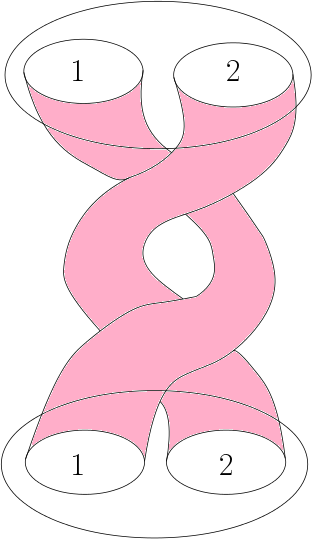
\includegraphics[scale=0.4]{Imagenes/generador}
	\caption{Generator of the fundamental group $\pi_1(E_2(2))=PB_2$, which also represents a homology class.}
\end{figure}

The operation $\mu$ induces an associative commutative product of degree 0  and $l$ essentially induces a Lie bracket of degree $1$. In fact, these two operations satisfy the axioms of a Gersternhaber algebra. Since both operations belong to $e_2(2)$ we can say that $e_2$ is generated by $e_2(2)$. What's more, those relations are sufficient to describe the operad $e_2$. That's why $e_2$ es sometimes called \emph{the operad of Gerstenhaber algebras}. %We will make precise the notion of generators and relations of an operad in the last chapter.


%PONER EN ALGUNA PARTE LA EQUIVALENCIA ENTRE ALGEBRAS DE GERSTENHABER Y ÁLGEBRAS SOBRE LA HOMOLOGÍA DEL OPERAD, A VER SI PUEDO DAR BIEN LA REFERENCIA ENTRE MAY Y COHEN, SI NO PREGUNTAR A MURO, SEGÚN ESTO ES COHEN \url{https://ncatlab.org/nlab/show/Gerstenhaber+algebra}


\end{document}

%isotopía \url{https://link.springer.com/chapter/10.1007%2F978-94-015-9319-9_6}
%Orientation preserving (que las cartas conservan la orientación) https://math.stackexchange.com/questions/1319234/meaning-of-the-expression-orientation-preserving-homeomorphism 
%O sea, conserva la orientación como superficie

%\url{https://math.mit.edu/~ebelmont/operads-talk.pdf}
%\url{http://math.uchicago.edu/~may/PAPERS/mayi.pdf}
%\url{https://neil-strickland.staff.shef.ac.uk/research/operads.pdf}